\documentclass[border=2mm]{standalone}

\usepackage{fontspec}
\usepackage{unicode-math}
\usepackage{amsmath}

\usepackage{pgfplots}
\pgfplotsset{compat=1.18}
\usetikzlibrary{arrows.meta, 
  calc, 
  positioning, 
  decorations.pathreplacing, 
  calligraphy}

\usepackage{xcolor}
\definecolor{den-1}{HTML}{111111}   % Đen #111111
\definecolor{den-2}{HTML}{222222}   % Đen #222222
\definecolor{den-3}{HTML}{333333}   % Đen #333333
\definecolor{den-4}{HTML}{444444}   % Đen #444444
\definecolor{den-5}{HTML}{555555}   % Đen #555555
\definecolor{den-6}{HTML}{666666}   % Đen #666666

% Thiết lập vị trí đặt nhãn gốc tọa độ
\tikzset{
  >=Stealth,
  originlabel/.style={
    font=\small\sf,
    anchor=north east, % Vị trí tương đối so với gốc
    yshift=-0.1ex,     % Điều chỉnh vị trí dọc một chút
    xshift=-0.1ex      % Điều chỉnh vị trí ngang một chút
  }
}

\begin{document}

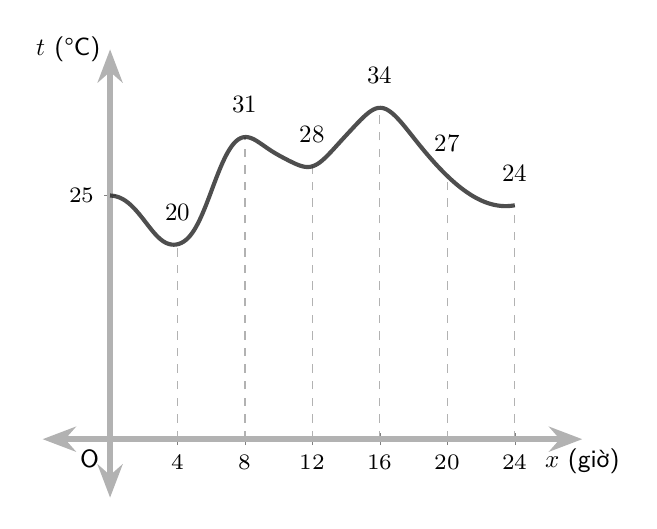
\begin{tikzpicture}

\begin{axis}[
    font=\small\sf,
    axis lines=middle,
    axis line style={<->, line width=2pt, color=den-6!50},
    xlabel={$x \text{ (giờ)}$},
    ylabel={$t \text{ (°C)}$},
    xlabel style={below, font=\small\sf},
    ylabel style={left, font=\small\sf},
    xmin=-4, xmax=28,
    ymin=-6, ymax=40,
    xtick={4, 8, 12, 16, 20, 24},
    ytick={25},
    tick label style={font=\footnotesize\sf, /pgf/number format/use comma=false, /pgf/number format/1000 sep={}},
    % xscale=1.5,
    clip=false,
]

\node[originlabel] at (axis cs:0,0) {O};

\draw [dashed, color=den-6!50] (4,0) -- (4,20);
\draw [dashed, color=den-6!50] (8,0) -- (8,31);
\draw [dashed, color=den-6!50] (12,0) -- (12,28);
\draw [dashed, color=den-6!50] (16,0) -- (16,34);
\draw [dashed, color=den-6!50] (20,0) -- (20,27);
\draw [dashed, color=den-6!50] (24,0) -- (24,24);

\node at (4,20) [anchor=south, yshift=5] {$20$};
\node at (8,31) [anchor=south, yshift=5] {$31$};
\node at (12,28) [anchor=south, yshift=5] {$28$};
\node at (16,34) [anchor=south, yshift=5] {$34$};
\node at (20,27) [anchor=south, yshift=5] {$27$};
\node at (24,24) [anchor=south, yshift=5] {$24$};


\addplot[smooth, line width=1.5pt, color=den-2, opacity=.8] coordinates {
  (0.000, 25.000)
  (0.080, 24.991)
  (0.161, 24.975)
  (0.241, 24.953)
  (0.321, 24.924)
  (0.401, 24.887)
  (0.482, 24.843)
  (0.562, 24.790)
  (0.642, 24.729)
  (0.722, 24.659)
  (0.803, 24.580)
  (0.883, 24.493)
  (0.963, 24.397)
  (1.043, 24.292)
  (1.124, 24.179)
  (1.204, 24.058)
  (1.284, 23.929)
  (1.365, 23.792)
  (1.445, 23.648)
  (1.525, 23.497)
  (1.605, 23.340)
  (1.686, 23.177)
  (1.766, 23.010)
  (1.846, 22.838)
  (1.926, 22.663)
  (2.007, 22.485)
  (2.087, 22.306)
  (2.167, 22.126)
  (2.247, 21.946)
  (2.328, 21.768)
  (2.408, 21.593)
  (2.488, 21.421)
  (2.569, 21.255)
  (2.649, 21.096)
  (2.729, 20.944)
  (2.809, 20.800)
  (2.890, 20.667)
  (2.970, 20.543)
  (3.050, 20.431)
  (3.130, 20.330)
  (3.211, 20.241)
  (3.291, 20.165)
  (3.371, 20.100)
  (3.452, 20.048)
  (3.532, 20.007)
  (3.612, 19.978)
  (3.692, 19.961)
  (3.773, 19.955)
  (3.853, 19.960)
  (3.933, 19.977)
  (4.013, 20.006)
  (4.094, 20.046)
  (4.174, 20.098)
  (4.254, 20.163)
  (4.334, 20.242)
  (4.415, 20.334)
  (4.495, 20.441)
  (4.575, 20.564)
  (4.656, 20.703)
  (4.736, 20.859)
  (4.816, 21.033)
  (4.896, 21.225)
  (4.977, 21.435)
  (5.057, 21.663)
  (5.137, 21.909)
  (5.217, 22.172)
  (5.298, 22.452)
  (5.378, 22.748)
  (5.458, 23.058)
  (5.538, 23.383)
  (5.619, 23.719)
  (5.699, 24.067)
  (5.779, 24.424)
  (5.860, 24.788)
  (5.940, 25.157)
  (6.020, 25.529)
  (6.100, 25.901)
  (6.181, 26.272)
  (6.261, 26.638)
  (6.341, 26.998)
  (6.421, 27.350)
  (6.502, 27.691)
  (6.582, 28.021)
  (6.662, 28.338)
  (6.742, 28.641)
  (6.823, 28.927)
  (6.903, 29.197)
  (6.983, 29.450)
  (7.064, 29.684)
  (7.144, 29.899)
  (7.224, 30.095)
  (7.304, 30.271)
  (7.385, 30.428)
  (7.465, 30.565)
  (7.545, 30.682)
  (7.625, 30.780)
  (7.706, 30.860)
  (7.786, 30.921)
  (7.866, 30.965)
  (7.946, 30.991)
  (8.027, 31.002)
  (8.107, 30.997)
  (8.187, 30.978)
  (8.268, 30.945)
  (8.348, 30.900)
  (8.428, 30.845)
  (8.508, 30.780)
  (8.589, 30.706)
  (8.669, 30.626)
  (8.749, 30.540)
  (8.829, 30.450)
  (8.910, 30.357)
  (8.990, 30.262)
  (9.070, 30.165)
  (9.151, 30.068)
  (9.231, 29.971)
  (9.311, 29.875)
  (9.391, 29.781)
  (9.472, 29.688)
  (9.552, 29.597)
  (9.632, 29.508)
  (9.712, 29.422)
  (9.793, 29.338)
  (9.873, 29.256)
  (9.953, 29.177)
  (10.033, 29.099)
  (10.114, 29.023)
  (10.194, 28.948)
  (10.274, 28.874)
  (10.355, 28.801)
  (10.435, 28.728)
  (10.515, 28.656)
  (10.595, 28.585)
  (10.676, 28.516)
  (10.756, 28.447)
  (10.836, 28.380)
  (10.916, 28.315)
  (10.997, 28.253)
  (11.077, 28.193)
  (11.157, 28.138)
  (11.237, 28.087)
  (11.318, 28.041)
  (11.398, 28.001)
  (11.478, 27.969)
  (11.559, 27.945)
  (11.639, 27.930)
  (11.719, 27.926)
  (11.799, 27.932)
  (11.880, 27.951)
  (11.960, 27.980)
  (12.040, 28.023)
  (12.120, 28.077)
  (12.201, 28.143)
  (12.281, 28.220)
  (12.361, 28.309)
  (12.441, 28.408)
  (12.522, 28.516)
  (12.602, 28.633)
  (12.682, 28.757)
  (12.763, 28.887)
  (12.843, 29.022)
  (12.923, 29.162)
  (13.003, 29.306)
  (13.084, 29.453)
  (13.164, 29.602)
  (13.244, 29.752)
  (13.324, 29.904)
  (13.405, 30.057)
  (13.485, 30.210)
  (13.565, 30.363)
  (13.645, 30.516)
  (13.726, 30.668)
  (13.806, 30.820)
  (13.886, 30.971)
  (13.967, 31.122)
  (14.047, 31.272)
  (14.127, 31.422)
  (14.207, 31.572)
  (14.288, 31.721)
  (14.368, 31.870)
  (14.448, 32.019)
  (14.528, 32.167)
  (14.609, 32.314)
  (14.689, 32.459)
  (14.769, 32.603)
  (14.849, 32.744)
  (14.930, 32.882)
  (15.010, 33.017)
  (15.090, 33.146)
  (15.171, 33.271)
  (15.251, 33.389)
  (15.331, 33.501)
  (15.411, 33.603)
  (15.492, 33.697)
  (15.572, 33.779)
  (15.652, 33.850)
  (15.732, 33.908)
  (15.813, 33.953)
  (15.893, 33.983)
  (15.973, 33.998)
  (16.054, 33.999)
  (16.134, 33.984)
  (16.214, 33.954)
  (16.294, 33.909)
  (16.375, 33.851)
  (16.455, 33.778)
  (16.535, 33.693)
  (16.615, 33.597)
  (16.696, 33.489)
  (16.776, 33.372)
  (16.856, 33.245)
  (16.936, 33.111)
  (17.017, 32.970)
  (17.097, 32.822)
  (17.177, 32.669)
  (17.258, 32.511)
  (17.338, 32.349)
  (17.418, 32.183)
  (17.498, 32.015)
  (17.579, 31.844)
  (17.659, 31.671)
  (17.739, 31.497)
  (17.819, 31.323)
  (17.900, 31.147)
  (17.980, 30.972)
  (18.060, 30.797)
  (18.140, 30.622)
  (18.221, 30.448)
  (18.301, 30.276)
  (18.381, 30.104)
  (18.462, 29.934)
  (18.542, 29.765)
  (18.622, 29.597)
  (18.702, 29.431)
  (18.783, 29.267)
  (18.863, 29.104)
  (18.943, 28.943)
  (19.023, 28.784)
  (19.104, 28.626)
  (19.184, 28.470)
  (19.264, 28.316)
  (19.344, 28.164)
  (19.425, 28.014)
  (19.505, 27.866)
  (19.585, 27.720)
  (19.666, 27.576)
  (19.746, 27.434)
  (19.826, 27.295)
  (19.906, 27.157)
  (19.987, 27.022)
  (20.067, 26.890)
  (20.147, 26.759)
  (20.227, 26.631)
  (20.308, 26.506)
  (20.388, 26.383)
  (20.468, 26.262)
  (20.548, 26.144)
  (20.629, 26.029)
  (20.709, 25.916)
  (20.789, 25.806)
  (20.870, 25.699)
  (20.950, 25.595)
  (21.030, 25.493)
  (21.110, 25.394)
  (21.191, 25.298)
  (21.271, 25.205)
  (21.351, 25.115)
  (21.431, 25.028)
  (21.512, 24.944)
  (21.592, 24.863)
  (21.672, 24.785)
  (21.753, 24.711)
  (21.833, 24.639)
  (21.913, 24.571)
  (21.993, 24.505)
  (22.074, 24.443)
  (22.154, 24.385)
  (22.234, 24.329)
  (22.314, 24.277)
  (22.395, 24.229)
  (22.475, 24.183)
  (22.555, 24.141)
  (22.635, 24.103)
  (22.716, 24.068)
  (22.796, 24.036)
  (22.876, 24.009)
  (22.957, 23.984)
  (23.037, 23.963)
  (23.117, 23.946)
  (23.197, 23.932)
  (23.278, 23.922)
  (23.358, 23.916)
  (23.438, 23.914)
  (23.518, 23.915)
  (23.599, 23.919)
  (23.679, 23.928)
  (23.759, 23.940)
  (23.839, 23.956)
  (23.920, 23.976)
  (24.000, 24.000)
};


\end{axis}

\end{tikzpicture}

\end{document}